\documentclass[a4paper]{article}
\usepackage{ifpdf}
\oddsidemargin=-5mm
\evensidemargin=-5mm\marginparwidth=.08in \marginparsep=.01in
\marginparpush=5pt\topmargin=-15mm\headheight=12pt
\headsep=25pt
\footskip=30pt
\textheight=25cm
\textwidth=17cm\columnsep=2mm
\columnseprule=1pt\parindent=15pt\parskip=2pt
\ifpdf
  % one of these two:
  \usepackage[pdftex]{graphicx}  % note the x at the end
  %\usepackage[pdftex]{epsfig}

  % hyperref should be the last package loaded:
  \usepackage[pdftex]{hyperref}
\else
  % one of these two:
  \usepackage[dvips]{graphicx}  % note the x at the end
  %\usepackage[dvips]{epsfig}

  % make the command \href from hyperref available as a 'print only'
  \newcommand{\href}[2]{#2}
\fi


\begin{document}
\begin{center}
\bf Semestralni projekt PAR 2007/2008:\\[5mm]
    Paralelni algoritmus pro reseni problemu UPO\\[5mm] 
       Miloslav Cinibulk\\
       Tomas Horacek\\[2mm]
5. rocnik, obor pocitace, K336 FEL CVUT, Karlovo nam. 13, 121 35 Praha 2\\[2mm]
\today
\end{center}

\section{Definice problemu a popis sekvencniho algoritmu}

\subsection{Vstupni data}
\begin{itemize}
	\item n = prirozene cislo
	\item k = prirozene cislo radu jednotek
	\item G = neorietovany neohodnoceny graf o n uzlech a stupni nejvyse k (zvolte standardni
	      reprezentaci s ocislovanymi uzly 1,...,n, napr. seznam sousedu nebo matici sousednosti).
	      Graf G nemusi byt souvisly.
\end{itemize}
\subsection{Ukol:}
Nalezt minimalni podmnozinu uzlu C, ktera pokryva kazdou hranu, tzn. kazda hrana je incidentni
s aspon s jednim uzlem z C.
\subsection{Vystup algoritmu:}
Vypis prvku mnoziny C (reseni existuje vzdy).
\subsection{Sekvencni algoritmus:}
Sekvencni algoritmus je BB-DFS s omezenou hloubkou prohledavaneho prostoru. Stav je dan obsahem
mnoziny C. Stav je pripustny, je-li C pokryti. Cena, kterou minimalizujeme, je $|$C$|$.
Pokryti C lze budovat bud pridavanim uzlu pocinaje prazdnou mnozinou, kdy se provadi navrat,
pokud jsou vsechny hrany pokryty, nebo odebiranim uzlu z nadbytecne velkeho pokryti, kdy se navrat
provadi, pokud nelze zadny uzel odebrat, aniz by se narusilo pokryti.

Dolni mez neni znama.

Trivialni horni mez $|$C$|$ je n/2.

Na zacatku algoritmu je nactena matice incidence grafu. Na zasobnik se vzdy ukladaji tato data:

\begin{itemize}
	\item cislo uzlu s kterym prave pracujeme
	\item to, zda odebirame uzel, nebo ponechavame uzel
	\item pocet zatim vybranych uzlu
	\item bitove pole vybranych uzlu
	\item pole hran s pocty uzlu s kterymi inciduji
\end{itemize}

Pocatecni stav algoritmu je takovy, ze jsou vybrany vsechny uzly. Pak algoritmus postupne zkousi
odebrat ruzne kombinace uzlu, ovsem vzdy tak, aby hrana kazda hrana incidovala alespon
s jednim uzlem (proto zasobnik obsahuje pole poctu uzlu incidujicich s jednotlivymi hranami).

Nejlepsi reseni se ukladaji do globalni promene a po projiti vsech smysluplnych kombinaci
odebrani uzlu se nejlepsi reseni vypise.

\section{Popis paralelniho algoritmu a jeho implementace v MPI}

Paralelni algoritmus je typu PBB-DFS-V. Princip algoritmu je stejny jako u sekvenciho reseni.

Na zacatku proces 0 nacte graf a rozesle ho ostatnim procesum. Prace se mezi procesi
rozesila formou polozky zasobniku. Po rozeslani grafu zacne proces 0 pocitat
a kdyz ma na zasobniku dostatecny pocet polozek pro vsechny procesy,
tak jim rozesle praci.

Behem vypoctu se muze stat, ze nektery proces dopocita svoje reseni. V tom pripade
se zepta sveho souseda, jestli mu nepreda cast prace a takto se pta v kruhu
dal, dokavad nejakou neziska.

Ukonceni paralelniho vypoctu je provedeno peskovymi algoritmem.

\section{Namerene vysledky a vyhodnoceni}

\subsection{Instance}

Instacemi byly 3 ruzne nahodne grafy se 70 uzly, kde 2 uzly maji stupen 30 a ostatni mensi.

\subsection{Namerene vysledky}

\begin{figure}[ht]
\centerline{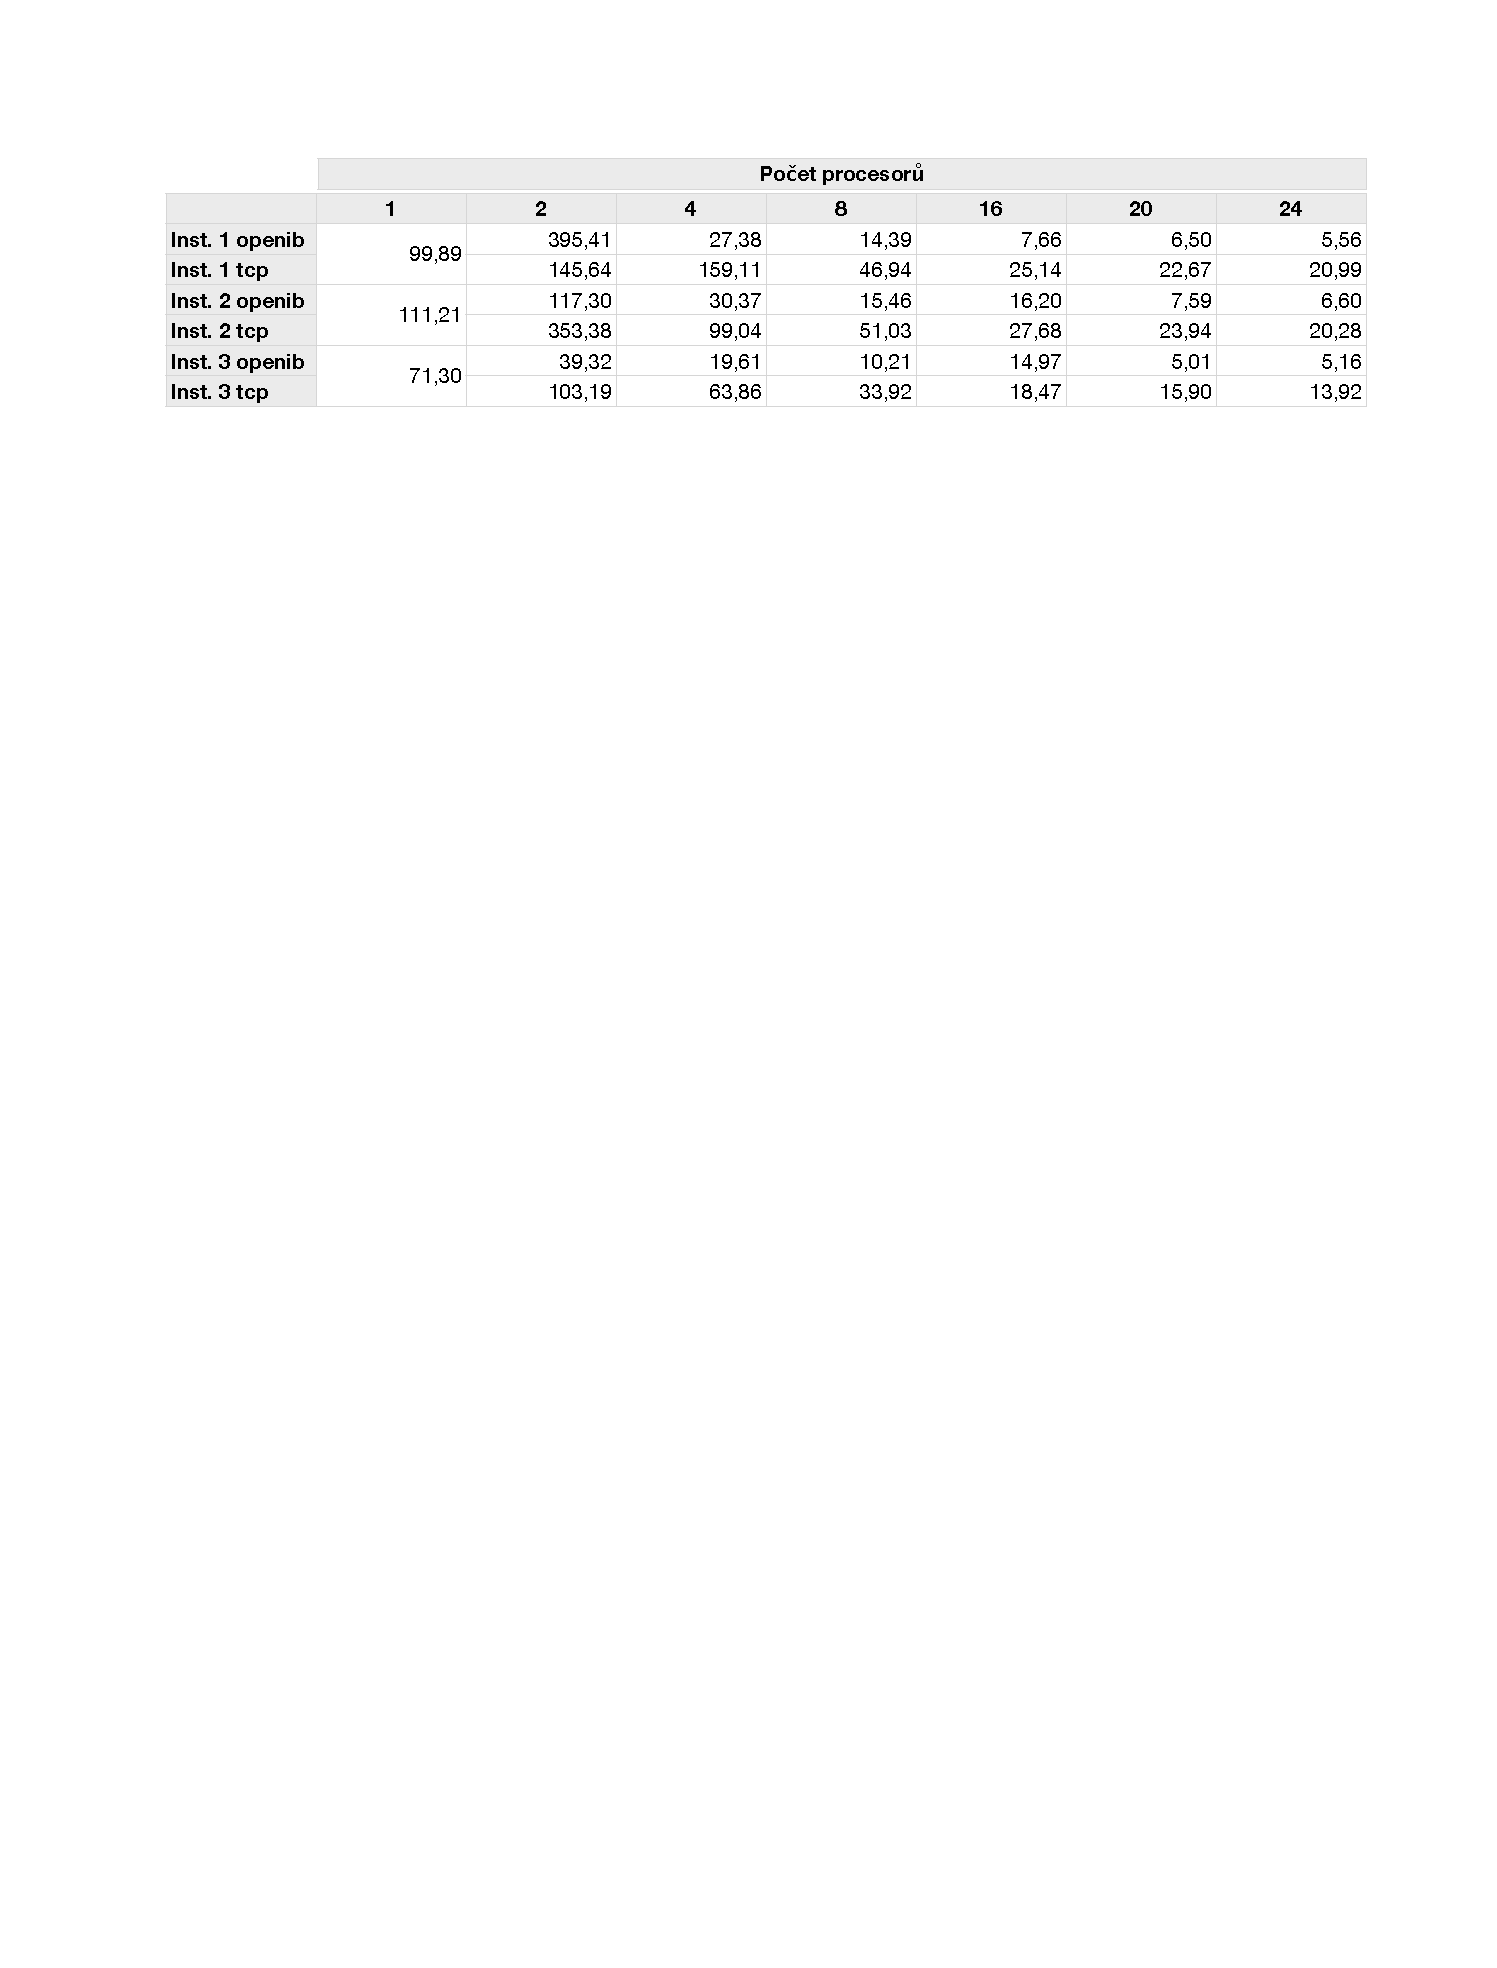
\includegraphics[width=\textwidth]{table-abs.pdf}}
\caption{Popis vaseho obrazku}
\label{table-abs}
\end{figure}

\begin{figure}[ht]
\centerline{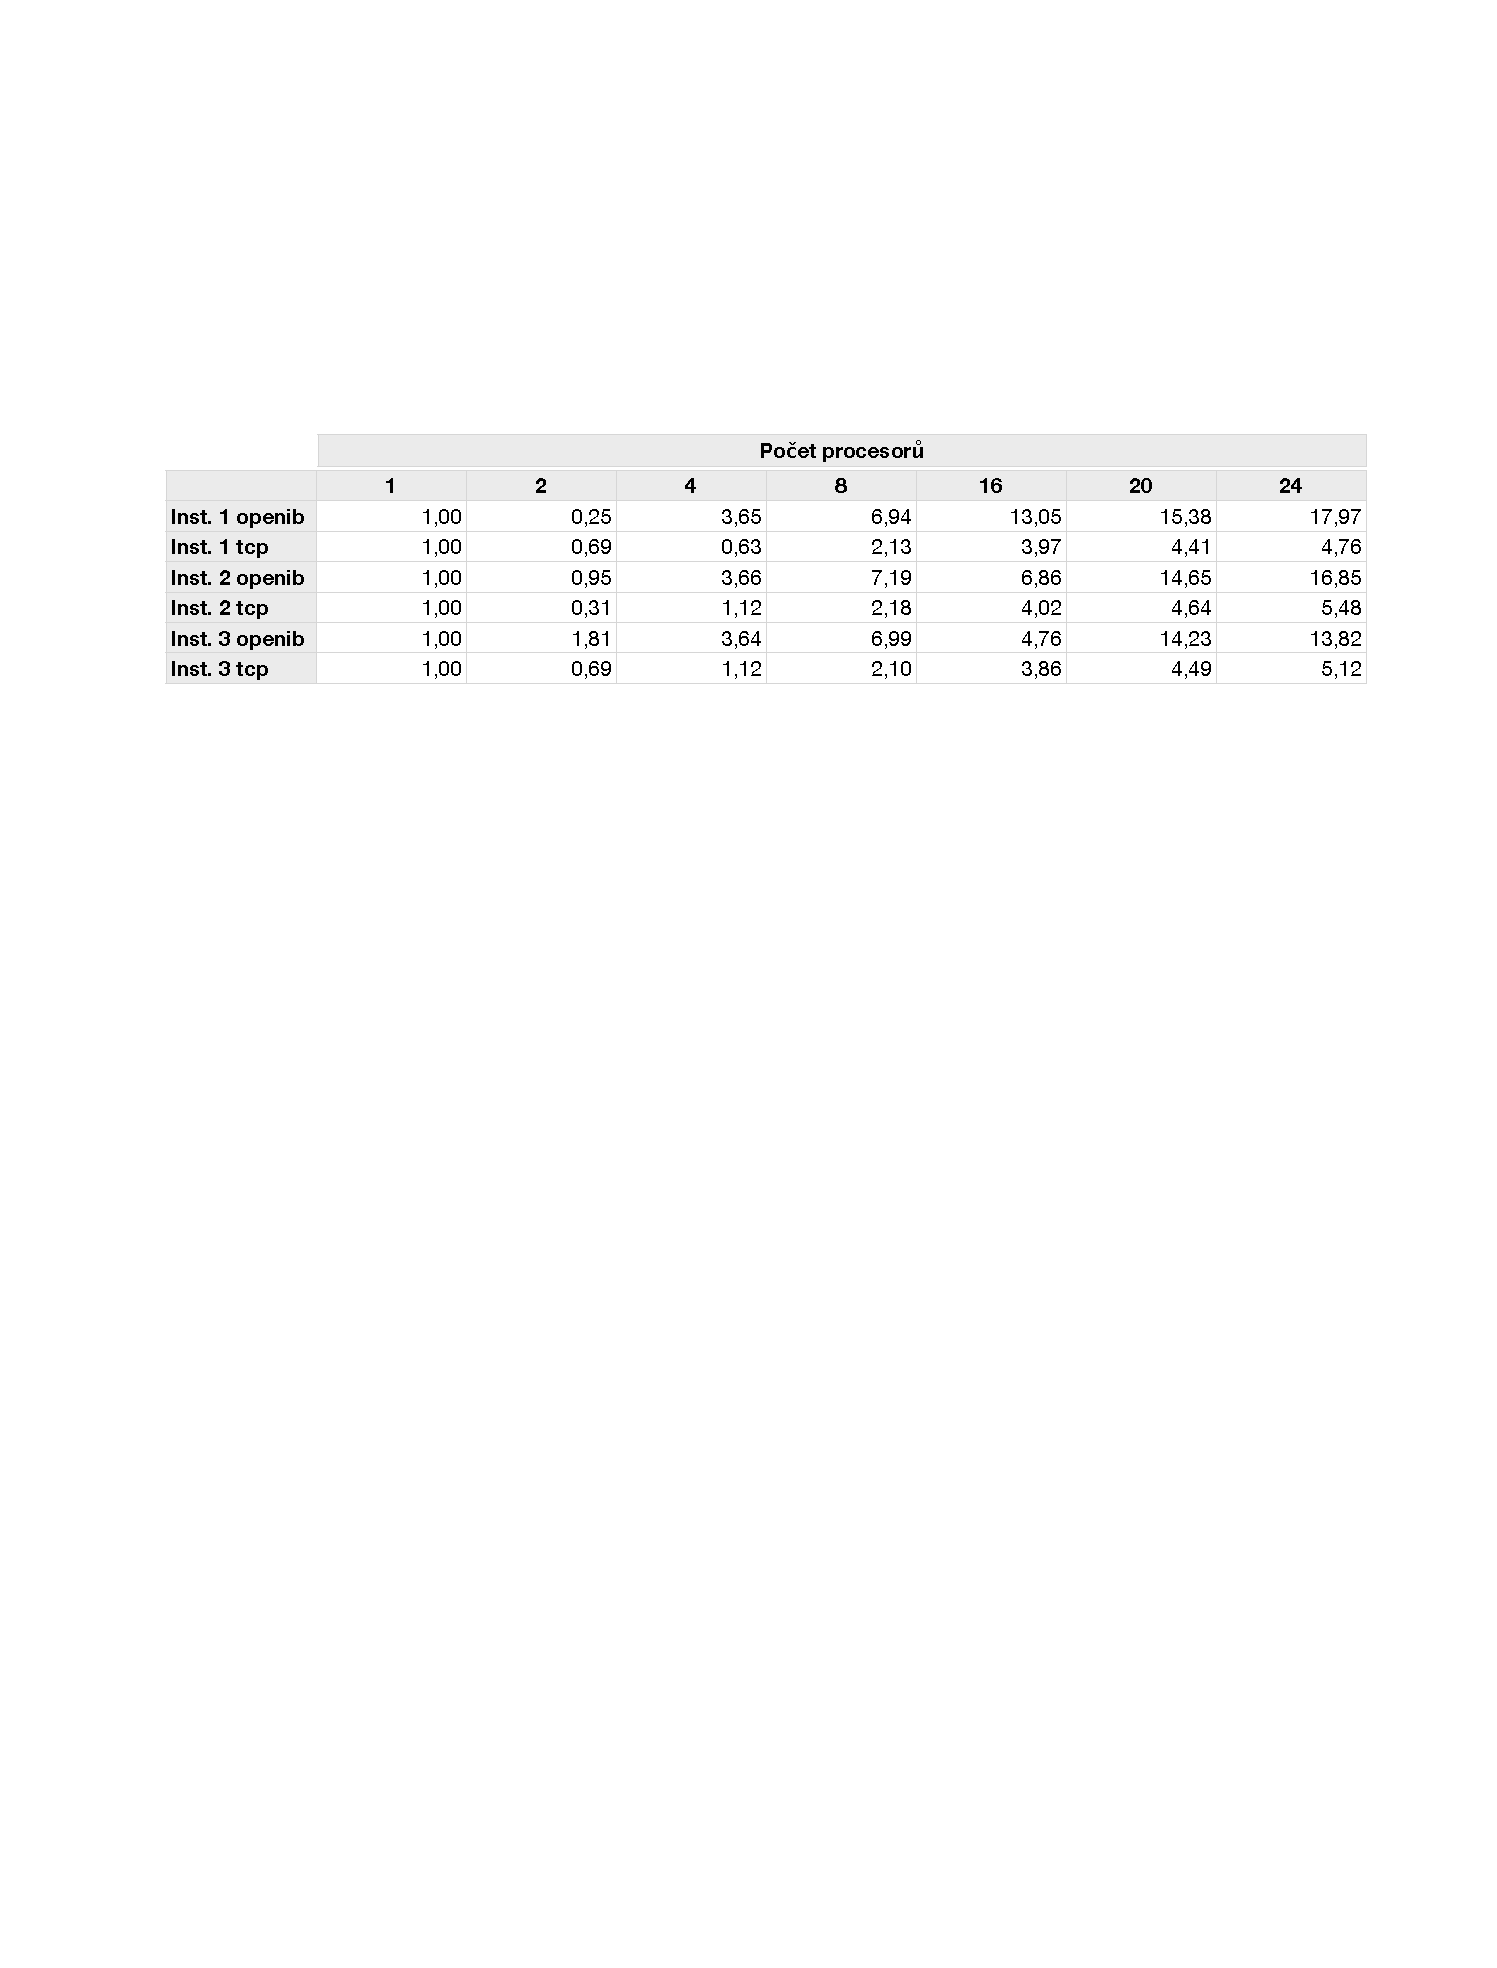
\includegraphics[width=\textwidth]{table-rel.pdf}}
\caption{Popis vaseho obrazku}
\label{table-rel}
\end{figure}

\begin{figure}[ht]
\centerline{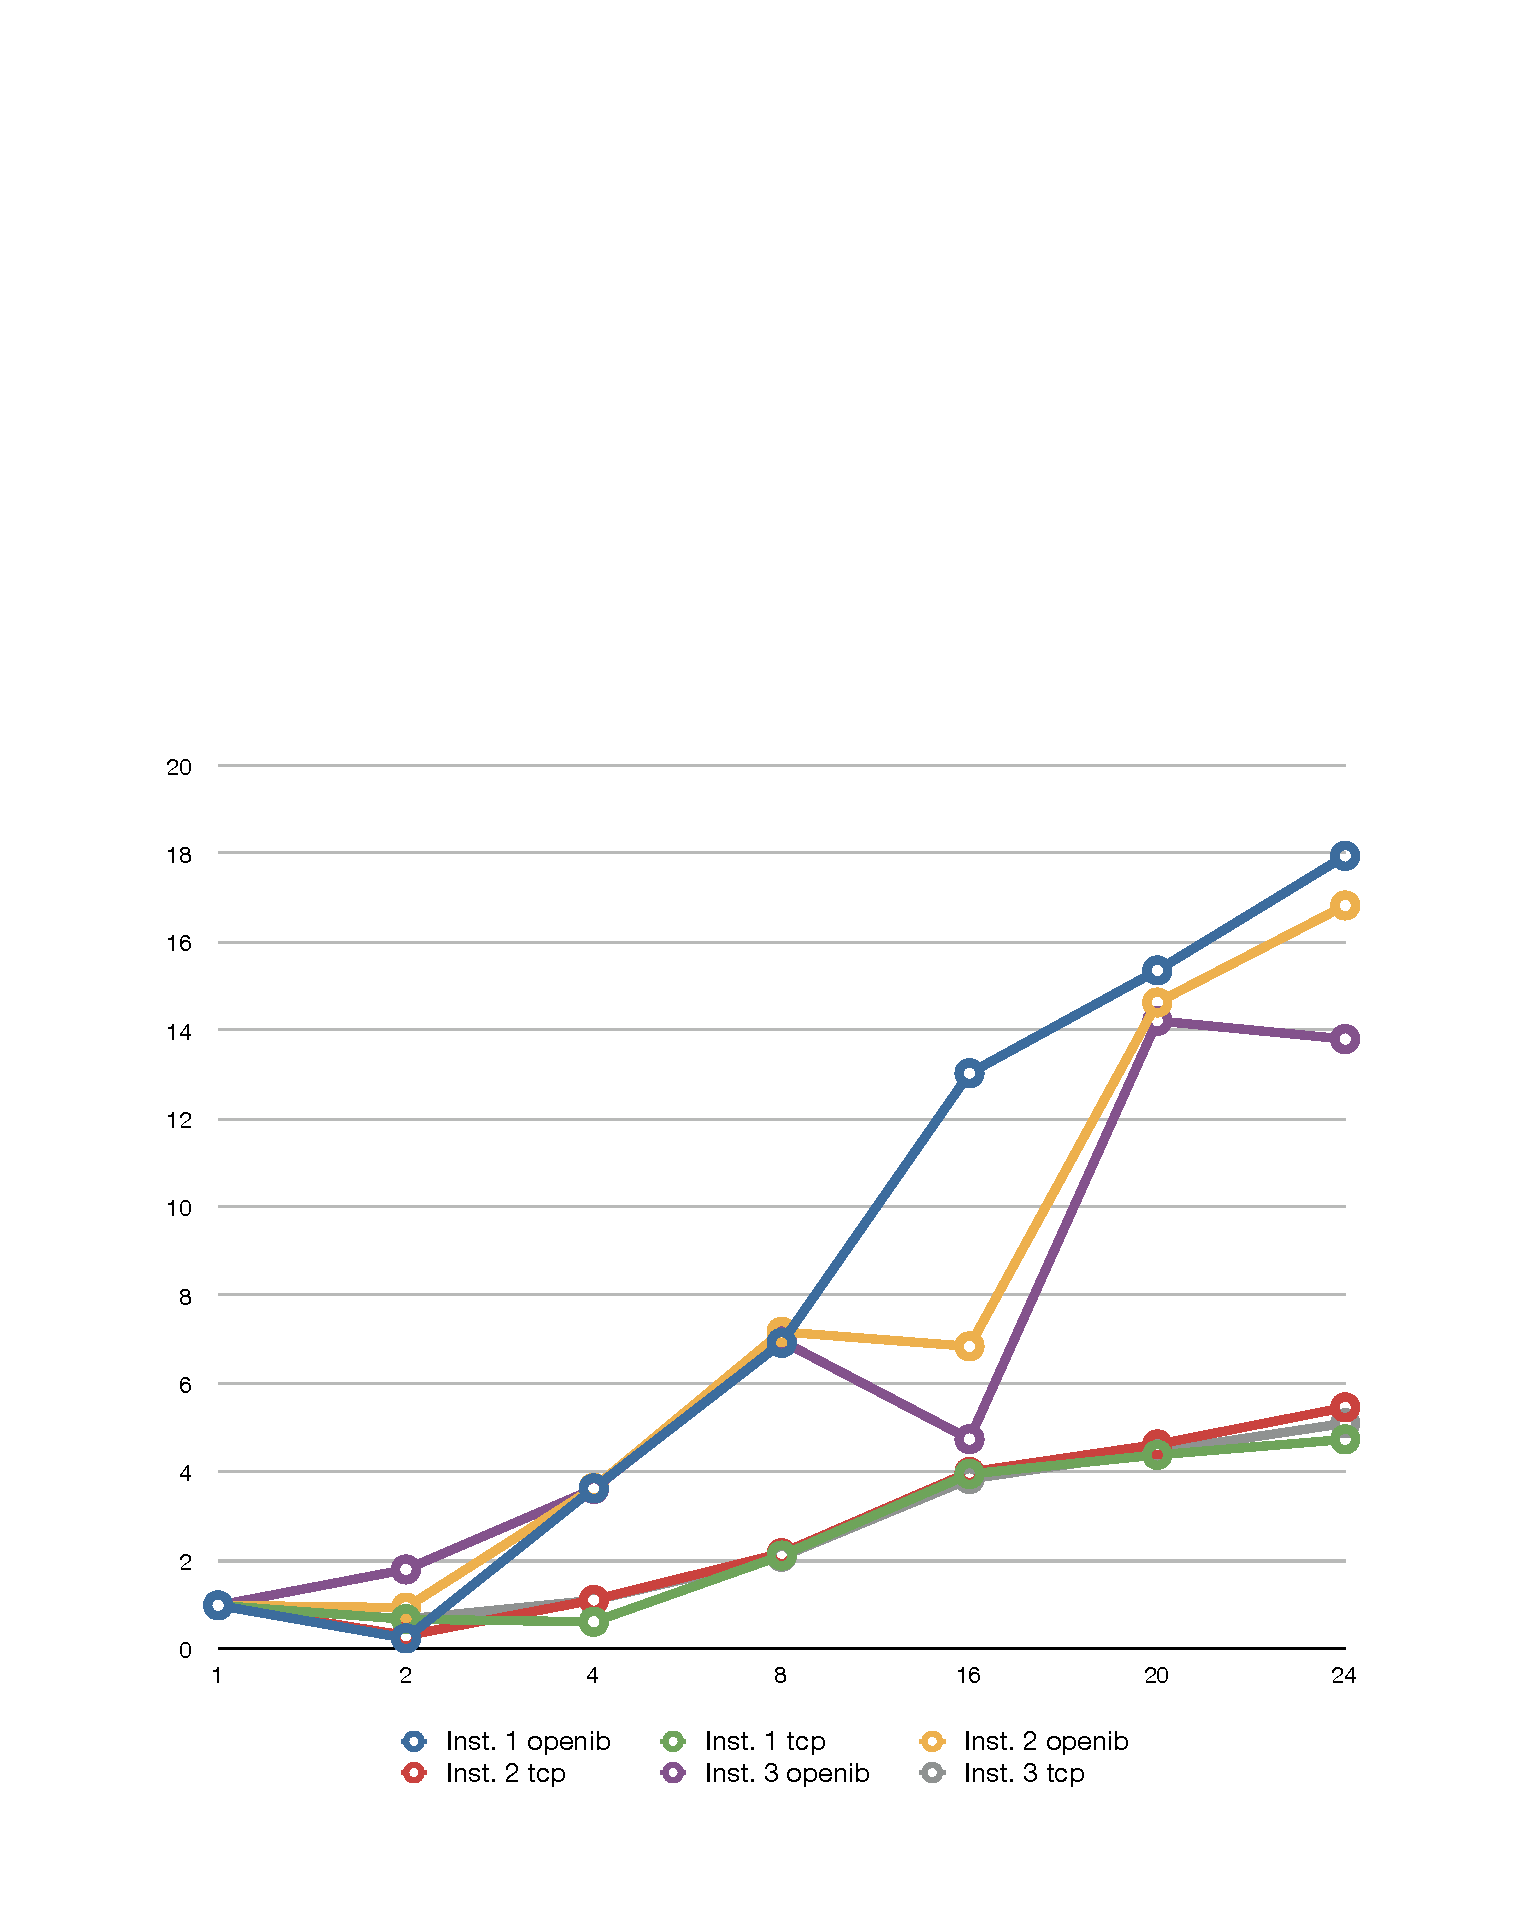
\includegraphics[width=\textwidth]{graph.pdf}}
\caption{Popis vaseho obrazku}
\label{labelvasehoobrazku}
\end{figure}

\begin{enumerate}
\item Zvolte tri instance problemu s takovou velikosti vstupnich dat, pro ktere ma sekvencni 
algoritmus casovou slozitost kolem 5, 10 a 15 minut.
Pro mereni cas potrebny na cteni dat z disku a ulozeni na disk neuvazujte a zakomentujte
ladici tisky, logy, zpravy a vystupy.
\item Merte paralelni cas pri pouziti $i=2,\cdot,24$ procesoru na sitich Ethernet a InfiniBand.
\item Z namerenych dat sestavte grafy zrychleni $S(n,p)$. Zjistete, zda a za jakych podminek
doslo k superlinearnimu zrychleni a pokuste se je zduvodnit.
\item Vyhodnodte komunikacni slozitost dynamickeho vyvazovani zateze a posudte
vhodnost vami implementovaneho algoritmu pro hledani darce a deleni zasobniku pri reseni vaseho
problemu. Posudte efektivnost a skalovatelnost algoritmu. Popiste nedostatky
vasi implementace a navrhnete zlepseni.
\item Empiricky stanovte 
granularitu vasi implementace, tj., stupen paralelismu pro danou velikost reseneho
problemu. Stanovte kriteria pro stanoveni mezi, za kterymi jiz neni
ucinne rozkladat vypocet na mensi procesy, protoze by komunikacni
naklady prevazily urychleni paralelnim vypoctem.

\end{enumerate}

\section{Literatura}

\appendix

\section{Navod pro vkladani grafu a obrazku do Texu}

Nejjednodussi zpusob vytvoreni obrazku je pouzit sunovsky graficky editor xfig,
ze ktrereho lze exportovat latex formaty (v poradi prosty latex, 
latex s macry epic, eepic, eepicemu) a postscript formaty,
uvedene poradi odpovida rustu komplikovanosti obrazku
(postscript umi jakykoliv obrazek, prosta latex macra pouze jednoduche,
epic makra neco mezi, je treba vyzkouset). Nasleduji priklady
pro vsechny pripady. 

Obrazek v postscriptu, vycentrovany a na celou sirku stranky, 
s popisem a cislem. Vsimnete si, jak ridit velikost obrazku.

Obrazek pouze vlozeny mezi radky textu, bez popisu a cislovani.\\
% \epsfxsize=1cm
% \rule{0pt}{0pt}\hfill\epsfbox{VasObrazek.ps}\hfill\rule{0pt}{0pt}

Texovske obrazky maji pripony *.latex, *.epic, *.eepic, a *.eepicemu, respective. 
% \begin{figure}[ht]
% \begin{center}
% \input VasObrazek.latex
% \end{center}
% \caption{Popis vaseho obrazku}
% \label{l1}
% \end{figure}
Vypustenim zavorek {\tt figure} dostanete opet pouze ramecek 
v textu bez cisla a popisu. 

Takhle jednoduse muzete poskladat obrazky vedle sebe.
% \begin{center}
% \setlength{\unitlength}{0.1mm}\input VasObrazek.epic
% \hglue 5mm 
% \setlength{\unitlength}{0.15mm}\input VasObrazek.eepic
% \hglue 5mm 
% \setlength{\unitlength}{0.2mm}\input VasObrazek.eepicemu
% \end{center}
Ridit velikost texovskych obrazku lze prikazem
\begin{verbatim}
\setlength{\unitlength}{0.1mm}
\end{verbatim}
ktere meni meritko rastru obrazku, Tyto prikazy je ale soucasne 
nutne vyhodit ze souboru, ktery xfig vygeneroval.

Pro vytvareni grafu lze pouzit program gnuplot, ktery umi generovat postscriptovy soubor, ktery vlozite
do Texu vyse uvedenym zpusobem.

\end{document}








